\chapter{Applications}\labch{applications}

In this chapter, we combine the path-tracing methods from \refch{path-tracing} with the differentiable formulations from \refch{drt} and the acceleration techniques from \refch{efficient-path-tracing} to demonstrate how these tools can be applied to real-world wireless-engineering problems. We focus on a canonical urban street canyon scenario, which is representative of many practical deployment environments, and we explore both forward modeling of the radio channel and inverse estimation problems.

\begin{figure}
  \centering
  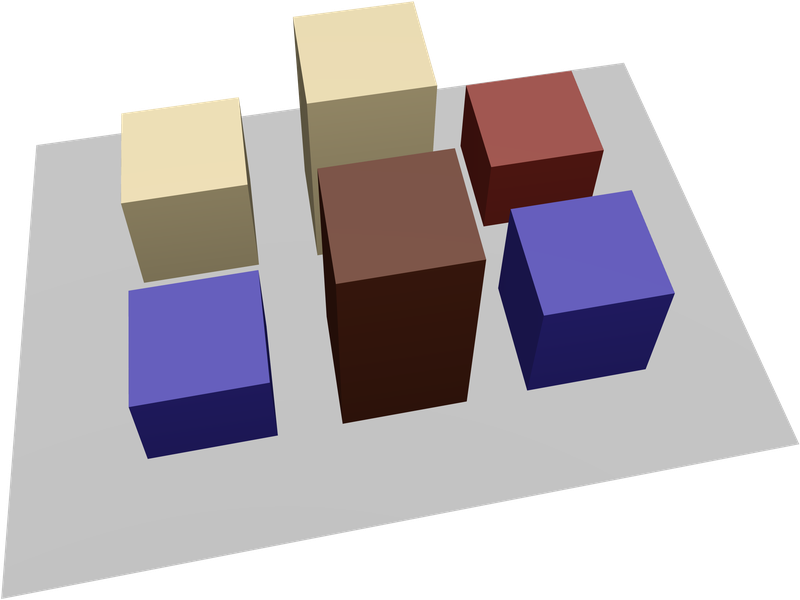
\includegraphics[width=.7\textwidth]{images/street-canyon.png}
  \caption{Simple street canyon scenario from Sionna~RT~\cite{Hoydis2023}.}
  \labfig{street-canyon}
\end{figure}

The urban street canyon scenario, illustrated in \reffig{street-canyon}, is a simple but representative environment for outdoor propagation in cities. It features a single street flanked by two rows of buildings, creating strong multipath propagation. It consists of 74 triangular facets: 12 per building (two facets per wall) and two for the ground. In the following sections, we focus on \gls{line-of-sight} and specular-reflection paths and, occasionally, diffraction paths to keep the analysis tractable. Due to the physical limitations of cascading multiple diffractions (discussed in \refsec{transition-regions}), we limit ourselves to first-order diffraction paths. However, the methods and insights presented here can be extended to more complex scenarios with additional propagation phenomena.

\section{Forward Modeling of the Radio Channel}

Forward modeling predicts radio-channel observables from known scene geometry, material properties, and network parameters. In practice, this is the core workflow for coverage analysis, network planning, and performance evaluation. Differentiable ray tracing extends this workflow by providing gradients of these observables with respect to both environment and system variables, as introduced in \refch{drt}. This enables not only simulation but also gradient-based design and calibration.

\subsection{Tracing of Propagation Paths}

The first task of a ray tracer is to identify physically valid propagation paths between a transmitter and a receiver, subject to geometric visibility constraints and electromagnetic interaction rules.

In the present example, we consider a single transmitter located on top of one building ($\bsup{x}_\text{\glsxtrshort{tx}} =
  \begin{bmatrix} -33 & 11 & 32
\end{bmatrix}^\top \unit{\meter}$), similar to a typical base-station location, and a receiver that can be placed anywhere in the scene at an altitude of \qty{1.5}{\meter}, representing a typical user-equipment height (e.g., a smartphone held in the user's hand). Because the transmitting antenna is placed on the roof of the building, the \gls{line-of-sight} path can be easily blocked, which further emphasizes the importance of simulating other propagation mechanisms such as reflections and diffractions. \reffig{street-canyon-paths} shows \gls{line-of-sight}, up to third-order reflection, and first-order diffraction paths found by the ray tracer for a receiver located at the center of the street, a typical user location in this scenario.

The left panel of \reffig{street-canyon-paths} highlights dominant \gls{line-of-sight} and specular-reflection trajectories, while the right panel isolates first-order diffraction paths around building edges. This decomposition is useful because it already reveals which mechanisms are likely to dominate in different street regions before any field computation is performed.

\begin{figure*}
  \centering
  \begin{subfigure}[t]{0.49\contentwidth}
    \centering
    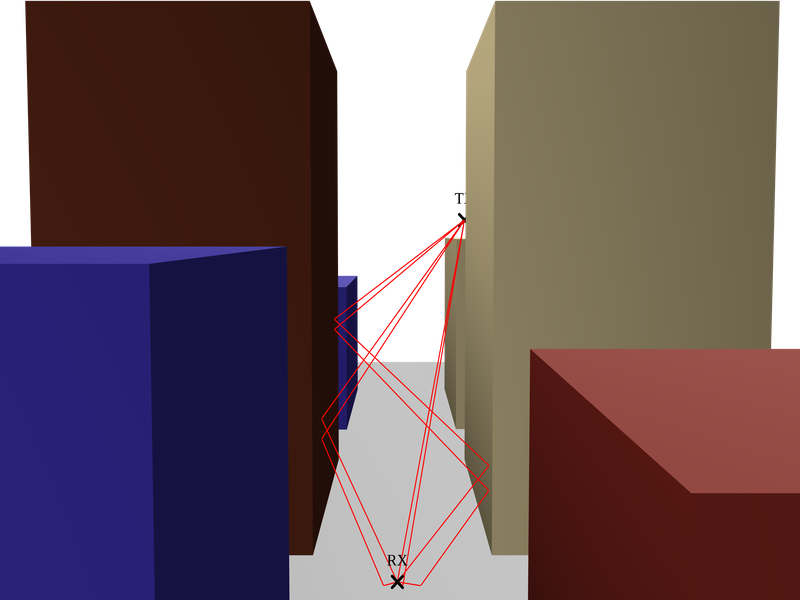
\includegraphics[width=\textwidth]{images/street-canyon-reflection-paths.png}
    \caption{\Gls{line-of-sight} and reflection paths.}
    \labfig{street-canyon-reflection-paths}
  \end{subfigure}
  \hfill
  \begin{subfigure}[t]{0.49\contentwidth}
    \centering
    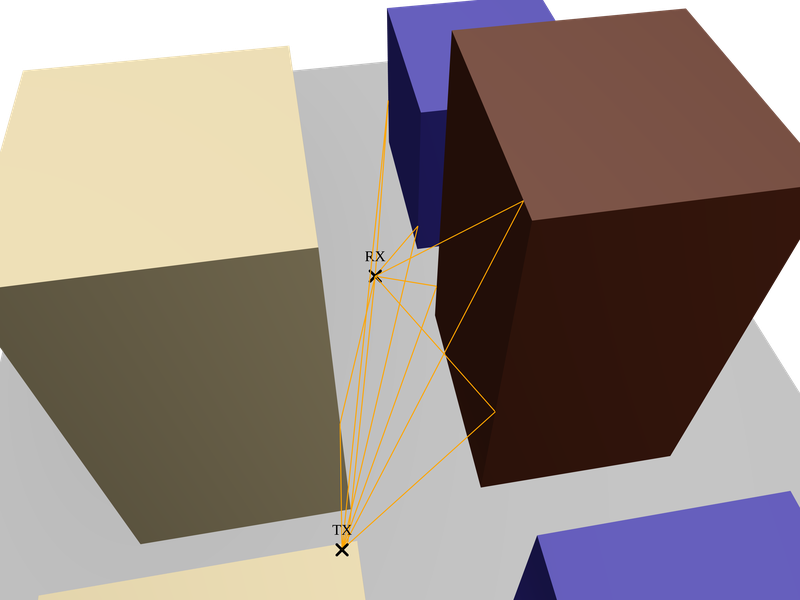
\includegraphics[width=\textwidth]{images/street-canyon-diffraction-paths.png}
    \caption{Diffraction paths.}
    \labfig{street-canyon-diffraction-paths}
  \end{subfigure}
  \caption{Propagation paths found by the ray tracer for a receiver located at the center of the street.}
  \labfig{street-canyon-paths}
\end{figure*}

Even before converting paths into channel coefficients, the geometric path set provides actionable information:
\begin{itemize}
  \item \emph{Multipath characterization} in which short, low-order interactions are typically the strongest contributors to received power.
  \item \emph{Physical interpretability}, since each path corresponds to a concrete mechanism (wall reflection, edge diffraction, etc.), which clarifies why channel behavior changes with geometry.
  \item \emph{Flexible propagation control} that allows selectively enabling or disabling specific propagation mechanisms to study their individual contributions, which is invaluable for validating models against measurements.
\end{itemize}

\subsection{From Paths to Channel Coefficients}

Once paths are identified, each interaction point is associated with an electromagnetic coefficient (reflection or diffraction), and the full per-path field transfer is assembled as described in \refch{rt-fundamentals} and \refch{path-tracing}. We consider a single transmitter--receiver link at \qty{28}{\giga\hertz}, with isotropic vertically polarized antennas. Scene materials are \enquote{concrete}, \enquote{glass}, \enquote{wood}, \enquote{marble}, and \enquote{brick} (ground, blue, brown, beige, and maroon buildings), with parameters from~\sidecite{ITU-R-P.2040}.

For each path $p$, we denote by $a_p \in \mathbb{C}$ the resulting complex scalar coefficient after interaction modeling, polarization projection, and antenna factors. The associated per-path power contribution is $|a_p|^2$ (up to the normalization adopted in \refch{rt-fundamentals}), which is the quantity used in the per-path gain plots below.

This conversion from geometric paths to complex coefficients provides several benefits:
\begin{itemize}
  \item \emph{Electromagnetic consistency} ensures that path delays, phases, interaction coefficients, and antenna responses are handled in one unified model.
  \item \emph{Interference fidelity} is preserved because constructive and destructive superposition emerge naturally from complex-path addition.
  \item \emph{Polarization handling} allows co- and cross-polarized components to be tracked separately when needed.
\end{itemize}

To model antenna arrays, two main approaches exist. The first approach is to run a single ray tracing simulation treating the array's phase center as a single point, and then reconstruct the response of each element by applying appropriate phase shifts. This phase correction is formalized through the use of steering vectors, which capture the relative phase delays across the array elements for a given path's direction of departure or arrival. Mathematically, a steering vector $\bsup{a}(\theta, \varphi) \in \mathbb{C}^M$ represents the relative phase shifts of a plane wave arriving at (or departing from) each of the $M$ elements of the array. For instance, for a uniform linear array of $M$ elements aligned along an axis with inter-element spacing $d_{a}$ and an arrival angle $\theta$ relative to the array broadside, the steering vector is expressed as
\begin{equation}
  \bsup{a}(\theta) =
  \begin{bmatrix} 1 & e^{-jk d_{a} \sin\theta} & \dots & e^{-jk d_{a} (M-1) \sin\theta}
  \end{bmatrix}^\top.
\end{equation}
By aggregating the relative phases, the steering vector maps the single-point ray tracing output to each individual antenna element. The second approach is to run multiple simulations, one per array element, and combine the results. The first approach is more efficient but less flexible, as steering vectors assume the incoming wave is locally planar across the entire array, which may fail to capture path-length differences or element-specific blockage. These effects can be significant for very large arrays or in environments where rays arrive at different angles for different elements. The second approach enables more detailed modeling of array geometry and mutual-coupling effects at the cost of increased computational load. The choice between these approaches depends on the specific application and required accuracy.

In the \gls{mimo} case, the scalar coefficient $a_p$ is therefore only a compact \gls{siso} abstraction. When the array response is kept explicit, the per-path contribution becomes matrix-valued and is naturally expressed through the outer product of the receive and transmit steering vectors, given by
\begin{equation}
  \bsit{H}_p(\tau) = a_p \bsup{a}_{\text{\glsxtrshort{rx}}}(\theta_p^{\text{\glsxtrshort{rx}}}, \varphi_p^{\text{\glsxtrshort{rx}}}) \bsup{a}_{\text{\glsxtrshort{tx}}}^{*}(\theta_p^{\text{\glsxtrshort{tx}}}, \varphi_p^{\text{\glsxtrshort{tx}}}) \delta(\tau - \tau_p),
\end{equation}
exactly as in the matrix-valued \gls{cir} introduced in \refsec{multipath-summation}. This outer product aggregates the individual multipath contributions across all transmit and receive element pairs.

\subsection{The Channel Impulse Response}

The paths and their associated coefficients are aggregated into a baseband \gls{cir} representation
\begin{equation}
  h(\tau) = \sum_{p=1}^{P} a_p\,\delta\left(\tau - \tau_p\right) \quad\text{with}\quad\tau_p = \frac{L_p}{c}.
\end{equation}
Here, $L_p$ is the path length and $c$ is the speed of light. Each impulse encodes one path delay, while its complex weight $a_p$ carries attenuation and phase.

The \gls{cir} bridges geometric ray tracing and communication-theoretic channel models. From $h(\tau)$, one can derive delay spread, coherence bandwidth, and frequency selectivity, all in a form directly consumable by link-level simulators.

To compare the individual contributions of reflection and diffraction mechanisms,
\reffig{reflection-diffraction-path-metrics} shows per-path amplitudes and gain as a function of delay.

\begin{figure*}
  \centering
  \inputtikz{path-amplitude-and-power}
  \caption{Per-path amplitude and gain versus delay for \gls{line-of-sight}, reflection, and diffraction paths in the urban street canyon scenario.}
  \labfig{reflection-diffraction-path-metrics}
\end{figure*}

\reffig{reflection-diffraction-path-metrics} confirms the expected structure: early-arriving \gls{line-of-sight} and reflection components dominate the received power, while diffraction contributes weaker but often critical delayed components that preserve connectivity in partially blocked configurations (see the coverage maps below for a more detailed view). The \gls{cir} representation provides several key benefits:
\begin{itemize}
  \item A \emph{direct link to signal processing}, since the \gls{cir} can be used immediately for equalization, modulation, and end-to-end communication-system simulation.
  \item A \emph{frequency-selectivity analysis} enabled by delay dispersion, which provides indicators such as $\tau_{\mathrm{RMS}}$ and approximate coherence-bandwidth scales.
  \item A \emph{mechanism-isolation capability}, where enabling or disabling \gls{line-of-sight}, reflection, or diffraction terms quantifies their separate impact.
\end{itemize}

\subsection{Handling Mobility}

With mobile users or dynamic environments, channel quantities become explicitly time dependent. Receiver and scatterer velocities induce Doppler shifts, which broaden the channel spectrum and reduce coherence time.

Two complementary simulation strategies are commonly used. A \emph{snapshot-based} approach repeatedly updates object positions and recomputes valid paths and coefficients. It is physically faithful and captures path birth/death events, but it is costly for long trajectories or fine temporal sampling. A \emph{Doppler-based} approach keeps the geometric path set fixed over a short window and applies analytical path-wise frequency shifts from object velocities. This approximation is much faster, but it remains accurate only while geometry changes are small (typically over a few \glspl{wavelength} of motion). In practice, the choice follows the required temporal horizon and fidelity.

\subsubsection{Doppler Shift and Frequency Translation}

For a propagation path $p$ with scattering points on moving objects, the accumulated Doppler shift is
\begin{equation}
  f_{p}^{\text{D}}(t) = -\frac{f_{\text{c}}}{c}\,\bsup{v}_{\text{\glsxtrshort{rx}}} \cdot \uvec{d}_p(t) - \frac{f_{\text{c}}}{c}\,\sum_i \bsup{v}_i \cdot \uvec{k}_i(t),
\end{equation}
where $\bsup{v}_{\text{\glsxtrshort{rx}}}$ is the receiver velocity, $\uvec{d}_p$ is the path arrival direction, $\bsup{v}_i$ is the velocity of the $i$-th scattering object, and $\uvec{k}_i$ is the outgoing ray direction at that point. The net Doppler shift depends on the relative velocities of transmitter, receiver, and all scattering surfaces. For the receiver, forward motion toward the transmitter induces positive (upward) frequency shifts, while receding motion induces negative shifts. The same pattern applies to each scattering surface along the path. Multiplying by the carrier frequency $f_{\text{c}}$ scales the shift: at millimeter-wave frequencies (\qty{28}{\giga\hertz}), a pedestrian traveling at \qty{5}{\meter\per\second} can incur Doppler shifts of hundreds of hertz per path, whereas at sub-\qty{6}{\giga\hertz} frequencies the shifts are correspondingly smaller.

\subsubsection{Coherence Time and Symbol-Rate Constraints}

A key implication of Doppler spread is the reduction of \emph{coherence time} $T_c$, i.e., the time interval over which the channel is approximately stationary. For Rician fading (when a dominant \gls{line-of-sight} component coexists with multipath scattering), a common approximation is
\begin{equation}
  T_c \approx \tfrac{0.423}{f_{\text{max}}^D},
\end{equation}
where $f_{\text{max}}^D$ is the maximum Doppler spread. When different paths carry different Doppler shifts, decorrelation accelerates and fewer symbols can reuse the same channel estimate. At high speeds or millimeter-wave carriers, coherence time may drop to microseconds, requiring frequent pilot updates and channel tracking. In low-mobility regimes, longer coherence times permit sparser channel-state-information feedback.

\subsubsection{Applications and Benefits}

Mobility-aware modeling provides several practical benefits:
\begin{itemize}
  \item A \emph{realistic temporal model} that captures user motion, traffic, and dynamic blockages explicitly, enabling handover analysis and beam-tracking studies.
  \item A \emph{Doppler-aware waveform-design workflow} using per-path frequency shifts to quantify spectral broadening and set pilot density, modulation mode, and channel-prediction strategy.
  \item A \emph{transient channel model} that reveals path appearance/disappearance and deep fades during short blockage events.
  \item A \emph{velocity-conditioned statistical perspective}, obtained by aggregating trajectories at different speeds to extract trends in Doppler spread, coherence time, and reliability.
\end{itemize}

\begin{figure}
  \inputtikz{receiver-power-mobility}
  \caption{The path gain of dominant \gls{line-of-sight}, reflection, and diffraction paths as a function of distance for a receiver moving along the street. The receiver starts at position $\bsup{x}_\text{\glsxtrshort{rx}} =
    \begin{bmatrix}25 & 0 & 1.5
  \end{bmatrix}^\top \unit{\meter}$ and moves away from the transmitter toward the positive $x$-direction.}
  \labfig{receiver-power-mobility}
\end{figure}

As shown in \reffig{receiver-power-mobility}, dominant components evolve smoothly but with distinct trends: the \gls{line-of-sight} term decreases with distance, reflection evolves nonlinearly due to incidence--reflection geometry, and diffraction remains weaker but structured. Even in a static urban scene, these mechanism-specific dynamics justify mobility-aware channel simulation.

\subsection{Coverage Maps}

\begin{figure*}
  \centering
  \begin{subfigure}[t]{0.49\contentwidth}
    \centering
    \import{pgf}{path-gain-reflection.pgf}
    \caption{Path gain from \gls{line-of-sight} and reflection paths.}
    \labfig{path-gain-reflection-paths}
  \end{subfigure}
  \hfill
  \begin{subfigure}[t]{0.49\contentwidth}
    \centering
    \import{pgf}{path-gain-diffraction.pgf}
    \caption{Path gain from diffraction paths.}
    \labfig{path-gain-diffraction-paths}
  \end{subfigure}
  \caption{Path-gain coverage maps for the street-canyon scenario, separating \gls{line-of-sight} and reflection contributions from diffraction contributions.}
  \labfig{path-gain}
\end{figure*}

Coverage maps---also referred to as radio maps---are obtained by evaluating channel-quality metrics over a dense grid of receiver positions. For each point $\bsup{x}$, ray tracing yields a \gls{cir}, from which received power, delays, \gls{sinr}, achievable rate, and outage are computed. Plotting these quantities as heat maps over the scene geometry reveals dead zones, dominant corridors, and deployment trade-offs.

As discussed in \refsec{multipath-summation}, these maps use the non-coherent addition of path powers, not the coherent summation of complex voltages. This convention suppresses small-scale fading and makes the maps more robust to tiny geometric perturbations, which is why it is the default for the coverage-map figures in this chapter.

\reffig{path-gain} highlights mechanism complementarity: the \gls{line-of-sight} and reflection coverage map exhibits corridor-like high-gain structures driven by specular visibility, while diffraction partially fills non-\gls{line-of-sight} regions with lower but useful power. Interpreting both maps jointly avoids overestimating coverage holes in specular-only analyses.

Furthermore, the diffraction-only coverage map in \reffig{path-gain-diffraction-paths} clearly shows the reflection and incident shadow boundaries (\glspl{rsb} and \glspl{isb}) in the diffracted power, as introduced in \refsec{shadow-boundaries}. Because the diffracted field in the \gls{utd} formulation is mathematically designed to compensate for the step discontinuities of the \gls{go} fields, the diffracted power itself exhibits sharp transitions and characteristic spatial patterns along these boundary lines.

Key metrics include the following definitions:
\begin{itemize}
  \item The \emph{coverage probability} is the fraction of the region with received power above a threshold,
    \begin{equation}
      p_{\mathrm{coverage}} = \frac{1}{|\mathcal{A}|} \int_{\mathcal{A}}\mathbb{I}\left[P_r(\bsup{x}) > P_{\min}\right] \mathrm{d}\bsup{x},
    \end{equation}
    where $\mathcal{A}$ is the region of interest and $P_{\min}$ is receiver sensitivity.
  \item The \emph{outage probability} is the fraction experiencing insufficient signal-to-interference-plus-noise ratio,
    \begin{equation}
      p_{\mathrm{outage}} = \frac{1}{|\mathcal{A}|} \int_{\mathcal{A}}\mathbb{I}\left[\mathrm{\gls{sinr}}(\bsup{x}) < \gamma_{\min}\right] \mathrm{d}\bsup{x},
    \end{equation}
    where $\gamma_{\min}$ is the minimum \gls{sinr} for reliable communication. This metric captures interference and noise, and therefore approximates usable (not only detectable) coverage.
  \item The \emph{rate coverage} is the fraction of the region capable of supporting a target data rate,
    \begin{wideequation}
      p_{\mathrm{rate}} = \frac{1}{|\mathcal{A}|} \int_{\mathcal{A}}\mathbb{I}\left[\log_2\!\big(1+\mathrm{\gls{sinr}}(\bsup{x})\big) > R_{\min}\right] \mathrm{d}\bsup{x},
    \end{wideequation}
    where $R_{\min}$ is the minimum required rate. This user-centric metric links propagation quality to service-level requirements.
\end{itemize}

Multi-frequency analyses are performed by repeating the same evaluation at each carrier frequency, thereby exposing frequency-dependent spatial heterogeneity.

Coverage-map-based analysis offers several practical benefits:
\begin{itemize}
  \item A \emph{visual planning aid} through heat maps that expose coverage gaps and candidate sites for base stations, relays, or beam reconfiguration.
  \item A \emph{quantitative benchmarking tool} based on area-level metrics for objective comparison between candidate deployments.
  \item A \emph{sensitivity-analysis capability} that recomputes maps under alternative assumptions (blockages, vegetation, antenna patterns) to reveal robustness limits.
  \item A \emph{backhaul co-design perspective} that uses visibility and coupling patterns to co-optimize access and backhaul placement.
\end{itemize}

\subsection{Optimizing Network Parameters}

A key advantage of differentiable ray tracing is that network parameters can be optimized directly with gradient-based solvers, avoiding exhaustive search and reducing reliance on heuristics.

\subsubsection{Optimizing Transmitter Orientation}

In practical deployments, antennas are directive and their orientation can be tuned to steer energy toward target regions. With differentiable ray tracing, gradients of coverage objectives with respect to orientation angles are available automatically, enabling efficient optimization.

Using Euler angles, the transmitter orientation is parameterized by three angles $\bsit{\theta} = (\alpha, \beta, \gamma)$ (roll, pitch, yaw). A common design objective is to maximize the average received power over a target region, i.e.,
\begin{equation}
  \bsit{\theta}^\star = \argmax_{\bsit{\theta}} \frac{1}{|\mathcal{A}|} \int_{\mathcal{A}} P_r(\bsup{x}; \bsit{\theta})\,\mathrm{d}\bsup{x},
\end{equation}
where $\mathcal{A}$ is the target area and the integral is approximated in practice by a receiver grid. Optimization is then performed with gradient-based methods (e.g., Adam~\sidecite{Kingma2015}) using automatic differentiation.

\begin{figure}
  \centering
  \inputtikz{optimization-antenna-orientation}
  \caption{Transmitter-orientation optimization: average received power (in \unit{\decibel}) and orientation-angle trajectories (roll, pitch, yaw) across optimization steps.}
  \labfig{orientation-optimization}
\end{figure}

In \reffig{orientation-optimization}, the objective increases smoothly from a random initial orientation, indicating stable convergence. Pitch and yaw show the dominant updates, while roll changes remain limited, consistent with beam steering primarily in elevation and azimuth. The optimized orientation yields a clear increase in the average received power over the target region.

\subsubsection{Optimizing Antenna Pattern}

Beyond orientation, the radiation pattern itself can be optimized. By tuning pattern-shape parameters, radiated energy can be redistributed to better match scene geometry and user distribution. Denoting the pattern parameters by $\bsit{\theta}$, we can find the antenna pattern that maximizes received power by solving
\begin{equation}
  \bsit{\theta}^{\star}
  = \argmax_{\bsit{\theta}} \sum_i P_r(\bsup{x}_i; \bsit{\theta}),
\end{equation}
where the sum is taken over a set of target receiver positions.

\begin{figure*}
  \centering
  \inputtikz{optimization-antenna-orientation-pattern}
  \caption{Antenna-pattern optimization: received power (in \unit{\decibel}) and learned pattern-direction angles (zenith and azimuth) across optimization steps.}
  \labfig{pattern-optimization}
\end{figure*}

This approach supports end-to-end antenna design for a specific deployment rather than generic isolated synthesis. For example, indoor reflective settings and outdoor street canyons induce different optimal patterns. Because the optimization includes scene materials and multipath, learned patterns are often better aligned with in-situ performance.

Representative use cases include the following examples:
\begin{itemize}
  \item A \emph{directional \gls{sinr} maximization} objective to optimize phased-array weights toward a user while suppressing known interferers.
  \item A \emph{scenario-specific compact MIMO design} approach to tailor a small-form-factor array to a target indoor or outdoor deployment.
  \item A \emph{null-steering strategy} to suppress dominant interferers while preserving useful multipath support.
\end{itemize}

\section{Inverse Problems}

Inverse problems reverse the standard simulation pipeline: instead of predicting measurements from a known scene, they infer unknown scene or system parameters from measured radio data. In wireless settings, these unknowns can include user position, material properties, antenna or network configuration, and even geometric scene structure. The practical value is substantial: once calibrated from observations, the same model can improve localization, reduce planning uncertainty, maintain digital twins over time, and support sensing tasks that are difficult with purely data-driven methods.

Historically, such formulations were often limited by non-convex objectives and expensive derivative computation. Differentiable ray tracing changes this by making the full forward model end-to-end differentiable, so gradients of the measurement mismatch with respect to physical parameters are obtained automatically and exploited by modern gradient-based optimizers. Combined with \gls{gpu} acceleration and automatic differentiation frameworks, this has made large-scale inverse optimization far more tractable and has driven strong recent interest in radio-frequency inverse sensing, including source localization~\sidecite[-13\baselineskip]{Han2025Loki,Han2025RayLoc,Lequeu2025}, material calibration~\sidecite{Hoydis2024,CastroFarfan2025}, and free-form 3D reconstruction with generative priors~\sidecite{Han2026}. We focus here on the first two applications, which are more mature and directly relevant to wireless communication.

\subsection{Inverse Localization}

Inverse localization estimates a receiver position by fitting a geometric model to radio observations collected from anchors at known locations. Unlike classical trilateration, which relies on idealized \gls{line-of-sight} distances, this formulation explicitly leverages multipath signatures, turning reflected and diffracted components into informative constraints rather than nuisance effects. This model-based approach also differs from \emph{radio fingerprinting}, which matches observed signatures against a precomputed database. While fingerprinting is robust in complex environments, it requires an expensive offline survey and is sensitive to scene changes. In contrast, differentiable ray tracing enables continuous optimization without a static database by solving the data-fitting problem
\begin{equation}
  \bsup{x}_\text{\glsxtrshort{rx}} = \argmin_{\bsup{x}} \sum_i \|y_i - \hat{y}_i(\bsup{x})\|^2,
\end{equation}
where $y_i$ represents measured channel features---such as power, time-of-arrival, or angle-of-arrival---and $\hat{y}_i(\bsup{x})$ denotes the corresponding ray tracing predictions for a candidate position $\bsup{x}$.

By providing gradients of the measurement mismatch via automatic differentiation, the framework enables efficient iterative updates toward a consistent position estimate. Although the resulting objective is typically non-convex and exhibits piecewise smoothness due to path-set transitions, smoothing strategies can effectively regularize the optimization landscape and improve convergence~\sidecite{Lequeu2025}.

In the example scenario, we consider three transmitters and one receiver. The reference position is
\begin{equation}
  \bsup{x}_\text{\glsxtrshort{rx}}^{\mathrm{ref}} =
  \begin{bmatrix} 10 & 0 & 1.5
  \end{bmatrix}^\top \unit{\meter},
\end{equation}
and the initialization is
\begin{equation}
  \bsup{x}_\text{\glsxtrshort{rx}}^{(0)} =
  \begin{bmatrix} 0 & -10 & 1.5
  \end{bmatrix}^\top \unit{\meter}.
\end{equation}

Multiple transmitters provide spatial diversity and richer multipath constraints. We minimize the mean squared error between measured and predicted received power over all transmitters. Iterative gradient updates converge to a local minimum, as shown in \reffig{inverse-localization-optimization}.

\begin{figure*}
  \centering
  \inputtikz{inverse-localization-optimization}
  \caption{Inverse-localization optimization: loss convergence and coordinate trajectories for the receiver position estimate.}
  \labfig{inverse-localization-optimization}
\end{figure*}

Ray-tracing-based inverse localization provides several key benefits:
\begin{itemize}
  \item A \emph{multipath-exploitation advantage} that retains useful accuracy in non-\gls{line-of-sight} settings where classical range-based methods degrade.
  \item An \emph{environment-awareness signal}, where mismatch patterns can indicate model drift (new obstacles, changed layouts) and trigger recalibration.
  \item A \emph{differentiable refinement and security-analysis workflow} that uses gradients for both joint model refinement and analysis of adversarial environmental perturbations~\sidecite{Han2025Loki}.
\end{itemize}

A few representative use cases include the following examples:
\begin{itemize}
  \item \emph{Indoor positioning} in warehouses, factories, and malls where satellite localization is unavailable.
  \item \emph{Emergency-response applications} that benefit from robust tracking in obstructed or damaged buildings with heavy multipath.
  \item \emph{Vehicular localization} in urban canyons, where satellite connectivity is intermittent and \gls{v2x} or cellular signals are informative.
\end{itemize}

\subsection{Radio Materials Calibration}

Radio-material calibration addresses a central modeling gap: electromagnetic parameters used in simulation are often uncertain, site dependent, and time varying. Relative permittivity, conductivity, and effective roughness directly shape reflection, absorption, and scattering, so even moderate parameter mismatch can produce a significant prediction error. The calibration objective is to recover these parameters from channel measurements by solving
\begin{equation}
  \bsit{\theta}_{mat}^\star = \argmin_{\bsit{\theta}_{mat}} \sum_i \|P_{\mathrm{meas},i} - \hat{P}_{\mathrm{sim},i}(\bsit{\theta}_{mat})\|^2,
\end{equation}
where $\bsit{\theta}_{mat}$ denotes candidate material parameters. Here, $P_{\mathrm{meas},i}$ is observed received power at location $i$, and $\hat{P}_{\mathrm{sim},i}(\bsit{\theta}_{mat})$ is the corresponding ray tracing prediction. Because the forward model is differentiable, gradients with respect to $\bsit{\theta}_{mat}$ are obtained automatically and used in efficient gradient-based solvers.

This differentiability also enables the joint fitting of not only material parameters but also antenna and scattering-model parameters from channel observations~\sidecite{Hoydis2024}.

Material calibration can be performed at multiple abstraction levels:
\begin{itemize}
  \item A \emph{per-material} calibration that fits one $\epsilon_r$ and $\sigma$ pair per material class (e.g., concrete, wood, glass).
  \item A \emph{per-surface} calibration that fits distinct parameters for non-uniform or weathered surfaces, with neural fields capturing continuous spatial variation.
  \item A \emph{frequency-dependent} calibration that performs separate or joint fitting across carrier frequencies to capture dispersion.
\end{itemize}

An illustrative calibration example, inspired by the Sionna~RT documentation \sidecite{Hoydis2023}, considers one unknown material (concrete) with unknown conductivity $\sigma$. Using a literature value as ground truth ($\sigma = \qty{0.63}{\siemens\per\meter}$), we minimize the mean squared error between measured and simulated received power over a single location. Starting from an arbitrary low conductivity, the optimization converges toward parameters that better match the observations, eventually reaching the ground truth (\reffig{material-calibration-optimization}).

\begin{figure}
  \centering
  \inputtikz{material-calibration-optimization}
  \caption{Radio-material calibration: loss convergence and estimated conductivity across optimization steps.}
  \labfig{material-calibration-optimization}
\end{figure}

Ray-tracing-based material calibration offers several benefits:
\begin{itemize}
  \item A \emph{reduction in uncertainty} from site-specific calibration that replaces coarse literature approximations.
  \item A \emph{digital-twin maintenance pathway} using periodic updates to track aging, moisture, and other environmental drifts.
  \item A \emph{lower measurement burden} by relying on non-intrusive channel measurements instead of direct material probing.
  \item A set of \emph{reusable fidelity gains} when calibrated parameters improve downstream studies across scenarios and frequencies.
\end{itemize}

Practical use cases for radio-material calibration include the following examples:
\begin{itemize}
  \item \emph{Indoor small-cell planning} that starts by calibrating venue-specific materials before optimizing placement, power, and interference control.
  \item \emph{Urban macro-cell planning} that builds representative city material libraries from multi-site calibration, including crowd-sourced data at scale~\sidecite{CastroFarfan2025}.
  \item \emph{Anomaly detection} using persistent simulation/measurement mismatch as an indicator of structural scene changes.
  \item \emph{Seasonal adaptation} relying on repeated calibration to track wet/dry and occupancy effects over time.
\end{itemize}

\subsection{System Constraints in Practical Deployments}

While the forward and inverse workflows demonstrate the power of differentiable ray tracing, their application in real-world networks is subject to several system-level constraints:
\begin{itemize}
  \item Tight \emph{latency budgets} in real-time radio resource management and beamforming control loops, which operate on millisecond timescales, make simulating a full 3D environment at each step computationally prohibitive, relegating ray tracing to offline planning or surrogate training.
  \item A carefully tuned \emph{measurement cadence} that dictates how quickly model drift (e.g., due to environmental changes or seasonal variation) can be detected and corrected, balancing the delay of recalibration against network overhead.
  \item Hard \emph{compute limits} from available hardware resources that constrain the spatial grid resolution for coverage maps, the number of propagation paths, and the interaction depth (e.g., limiting diffraction to one bounce) to avoid memory and execution bottlenecks, particularly in reverse-mode automatic differentiation.
  \item Inherent \emph{accuracy--cost trade-offs} when choosing modeling options (e.g., whether to include diffuse scattering or detailed antenna patterns), forcing engineers to select physical mechanisms based on the accuracy requirements of the specific application.
\end{itemize}

\section{Conclusion}

This chapter has illustrated the practical scope of differentiable ray tracing in both forward and inverse workflows. On the forward side, geometric scene descriptions and network settings are converted into channel observables such as \glspl{cir}, received power, and coverage maps. Because these quantities are differentiable, the transmitter pose, orientation, and pattern parameters can be optimized with gradient-based solvers instead of trial-and-error tuning. Mobility modeling further extends this pipeline to time-varying channels and Doppler-aware performance analysis.

On the inverse side, localization and material calibration show how measurements can be fused with simulation to infer latent variables and maintain accurate digital twins. Multipath-aware localization improves robustness in the absence of a direct \gls{line-of-sight} path, while calibration adapts material parameters as deployments evolve. Together, these inverse workflows close the loop between prediction and observation.

While ray tracing techniques are mainly used for offline planning and analysis, their online deployment remains shaped by practical constraints. \emph{Latency budgets} limit the direct use of full ray tracing in real-time control loops, motivating surrogate models. \emph{Measurement cadence} determines how quickly model drift can be detected and corrected. \emph{Compute limits} constrain spatial/angular resolution and propagation richness, requiring selective model complexity. \emph{Accuracy--cost trade-offs} therefore remain central when deciding which mechanisms to include for a given application.

These trade-offs determine whether a workflow is best run offline (planning), periodically (recalibration), or in near real time via learned approximations. The next chapter (\refch{research-applications}) builds on this foundation with learning-assisted path search for scalability and multipath-lifetime analysis for transient behavior.
